%!TEX root = ../thesis.tex
%*******************************************************************************
%****************************** Third Chapter **********************************
%*******************************************************************************
\chapter{Planificación y estado de avance.}

% **************************** Define Graphics Path **************************
\ifpdf
    \graphicspath{{Chapter5/Figs/Raster/}{Chapter5/Figs/PDF/}{Chapter5/Figs/}}
\else
    \graphicspath{{Chapter5/Figs/Vector/}{Chapter5/Figs/}}
\fi

Es posible pensar en este proyecto de Tesis, como un conjunto de postulaciones y planteamientos de nuevas metodologías basadas en el uso de técnicas de minería de datos que permitan estudiar mutaciones en conjuntos de datos y que culminan con una gran temática, que aborda la implementación de una herramienta computacional para el diseño de mutaciones.

Dado esto, el proyecto en sí, puede dividirse en tres grandes objetivos, de los cuales, los conocimientos y destrezas adquiridas en los primeros dos, son necesarias para cumplir con el tercer gran objetivo. Esto, es posible observarlo en la Figura \ref{cap5:fig1}.

\begin{figure}[!h]
	
	\centering
	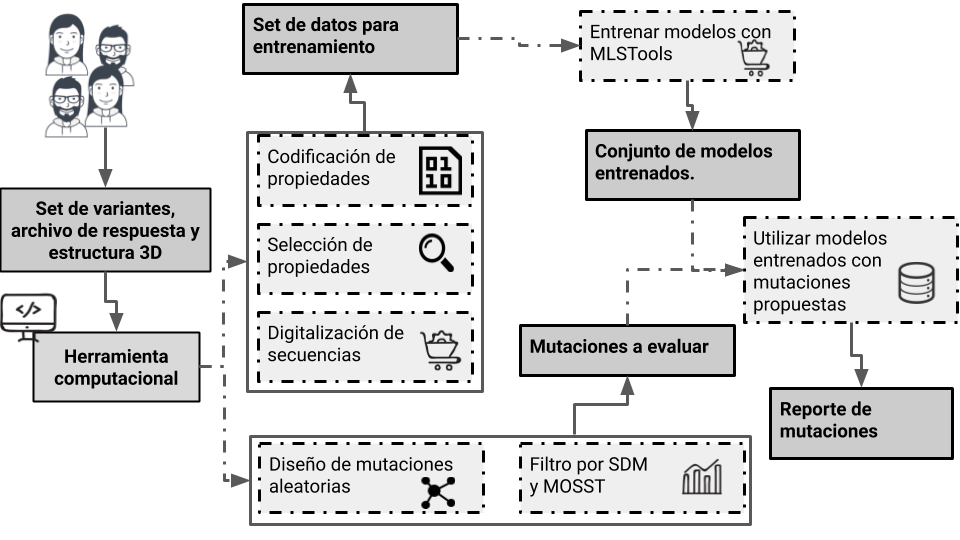
\includegraphics[scale=.5]{fig1.png}
	\caption{Esquema representativo de objetivos generales involucrados en el desarrollo del proyecto.}
	\label{cap5:fig1}
\end{figure}

El primer objetivo, se basa en la construcción de modelos de clasificación o regresión basados en algoritmos de aprendizaje supervisado, enfocados en el estudio de mutaciones puntuales en una proteína y cómo afectan éstas en términos de una respuesta conocida, como por ejemplo, estabilidad, productividad, actividad, etc. Esto, va en directo beneficio del estudio de nuevas mutantes o variantes en proteínas de interés, apoyados en una metodología que maximiza el desempeño de los modelos y sin incurrir en costos computacionales elevados. No obstante, el hecho de manipular nuevas mutaciones, requiere una verificación experimental. Sin embargo, esto permite minimizar los costos económicos y de recursos humanos que conlleva estudiar un gran conjunto de espacios muestrales de mutaciones. 

Por otro lado, el segundo objetivo se basa principalmente en representar secuencias lineales de proteínas a partir de la digitalización de propiedades fisicoquímicas y empleando transformadas de Fourier como representación de espectros de frecuencias. Si bien, el enfoque principal es la representación en sí, el objetivo también abarca el cómo utilizar estas representaciones para el entrenamiento de modelos de clasificación/regresión o el reconocimiento de patrones e identificación de residuos que aportan a las propiedades fisicoquímicas.

Finalmente, el tercer gran objetivo, comprende el desarrollo de una herramienta computacional, basada en técnicas de minería de datos para el diseño de mutaciones en proteínas de interés. El cómo se abarcará esta problemática, comprende, por un lado, definir representaciones de las secuencias lineales y cómo codificar sus propiedades fisicoquímicas, en conjunto, con el entrenamiento de modelos de clasificación/regresión que permitan evaluar nuevas mutantes. Es decir, los enfoques propuestos en los capítulos \ref{cap3} y \ref{cap2}, respectivamente. Demostrando así, las relaciones existentes entre cada capítulo y cómo estos apuntan a un objetivo general que conlleva aplicar minería de datos en el estudio de mutaciones puntuales asociados a la ingeniería de proteínas.

Con el fin de trazar los panoramas asociados al desarrollo de cada metodología y exponer el estado de avance del proyecto en cuanto a las diferentes actividades desarrolladas, en el presente capítulo, se expone un conjunto de actividades resumen de cada objetivo, asociados a un tiempo estimativo que conlleva el cumplimiento de estos y a su vez, el estado de avance actual, junto con los objetivos siguientes a tratar.

\section{Planificación}

La planificación se centra en cumplir los tres grandes objetivos y se plantea una estimación del tiempo que conlleva el desarrollo de cada una de las temáticas. Se exponen diferentes tareas generales que aportan a cumplir los objetivos y el tiempo estimativo, considerando un desarrollo general de 3 años como máximo.

\section{Estado de avance}




